\chapter{Brass}\label{ch:brass}

\SWcomment[terms I could use: bore, tube, cylinder]

In this work, the wave propagation in tubes is approximated using a 1D system

\section{Webster's Equation}

The main difference between the 1D brass PDE and the 1D wave equation is the presence of a variable cross-section. For low-amplitude vibrations in an (axially symmetric) acoustic tube and for which the wavelengths are much larger than the radius of this tube, one can describe its dynamics using \textit{Webster}'s equation \cite{Webster1919}
\begin{equation}\label{eq:webstersPDE}
    S\partial_t^2\Psi = c^2\partial_x(S\partial_x\Psi),
\end{equation}
with \textit{acoustic potential} $\Psi = \Psi(x,t)$ (in m$^2$/s), $S = S(x)$ is the cross sectional area (in m$^2$) and the speed of sound in air $c$ (in m/s). If $S(x) = 1$ for all values of $x$, Eq. \eqref{eq:webstersPDE} reduces to the 1D wave equation in Eq. \eqref{eq:1DwavePDE}. The acoustic potential can be related to pressure $p = p(x,t)$ (in Pa) and particle velocity $v = v(x,t)$ (in m/s) according to
\begin{equation}
    p = \rho \pt \Psi, \qaq v = -\px \Psi.
\end{equation}


\subsection{Discretisation}
Introducing interleaved gridpoints at $n-1/2$ and $n+1/2$ for $S$, a we can discretise Eq. \eqref{eq:webstersPDE} (following \cite{Bilbao2018}) to
\begin{equation}\label{eq:discWebster}
    \Sbar \delta_{tt}\Psi^n_l = c^2\dxp(\Sm(\delta_{x-}\Psiln)),
\end{equation}
where
\begin{equation}
    \Sbar = \mxp\Sm = \frac{\Sp + \Sm}{2}.
\end{equation}
The right side of the equation in \eqref{eq:discWebster} contains an operator applied to two grid functions ($S$ and $\Psi$) multiplied onto each other. In order to expand this, we need to use the product rule (Eq. (2.23) in \cite{theBible}) which is
\begin{equation}
    \dxp (u_lw_l) = (\dxp u_l)(\mxp{w_l}) + (\mxp u_l)(\dxp w_l).
\end{equation}
In the case of \eqref{eq:discWebster}, $u_l \triangleq \Sm$ and $w_l \triangleq \dxm\Psiln$. Expanding (retaining the notation for $\Sbar$) and solving for $\Psinp$ yields (Appendix \ref{app:webstersUpdateEq})
\begin{equation}
    \Psinp = 2(1-\lambda^2)\Psiln-\Psinm+ \frac{\lambda^2\Sp}{\Sbar}\Psilp + \frac{\lambda^2\Sm}{\Sbar}\Psilm,\label{eq:webstersUpdateEq}
\end{equation}
which is identical to Eq. (19.51) in \cite{Bilbao2018}.
Also see Figure \ref{fig:variableCrossSection}

\begin{figure}[h]
    \centering
    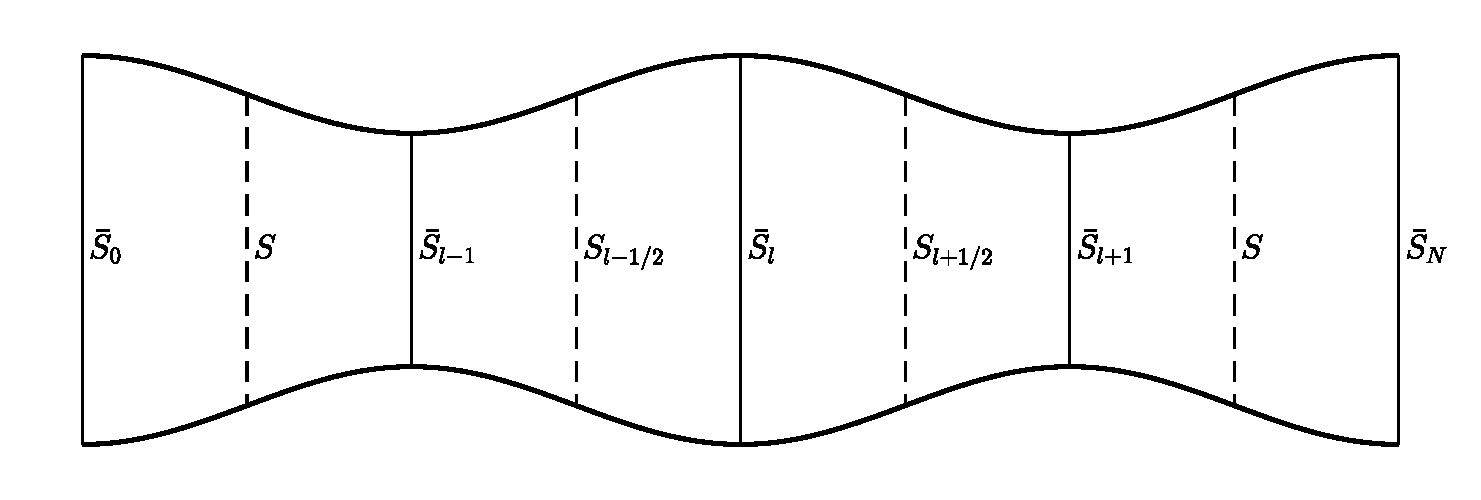
\includegraphics[width=0.9\textwidth]{figures/resonators/variableCrossSection.eps}
    \caption{Approximations to $S(x)$..\SWcomment[left off here!] \label{fig:variableCrossSection}}
\end{figure}

\subsection{Boundary Conditions}
The choices for boundary conditions in an acoustic tube are open and closed, defined as \cite{Bilbao2018}
\begin{equation}
    \begin{split}
        \partial_t\Psi &= 0\ \text{(open, Dirichlet)}\\
        \partial_x\Psi &= 0\ \text{(closed, Neumann)},
    \end{split}
\end{equation} 
at the ends of the tube. This might be slightly counter-intuitive as in the case of a string ``closed" might imply the ``clamped" or Dirichlet boundary condition. The opposite can be intuitively shown imagining a wave front with a positive acoustic potential moving through a tube and hitting a closed end. What comes back is also a wave front with a positive acoustic potential, i.e., the sign of the potential does not flip, which also happens using the free or Neumann condition for the string.

In this case we follow \cite[Chapter 9]{theBible} and use the following
\begin{equation}\label{eq:openClosed}
    \partial_x\Psi(0, t) = 0 \quad \text{and} \quad \partial_t\Psi(L, t) = 0
\end{equation}
i.e. closed at the left end and open at the right end. In discrete time we have two choices for the closed condition
\begin{equation}\label{eq:centNonCentBound}
\begin{split}
    \delta_{x\cdot}\Psi_0^n &= 0 \ \Rightarrow \ \Psi_{-1}^n = \Psi_1^n \quad \text{(centered)}\\
    \delta_{x-}\Psi_0^n &= 0\  \Rightarrow \ \Psi_{-1}^n = \Psi_0^n\quad \text{(non-centered)}
\end{split}
\end{equation}
At the left boundary we can now solve Eq. \eqref{eq:webstersUpdateEq} for the centered case:
\begin{equation}
    \begin{aligned}
        \Psi_0^{n+1} &= 2(1-\lambda^2)\Psi_0^n-\Psi_0^{n-1}+ \frac{\lambda^2S_{1/2}}{\bar S_0}\Psi_1^n + \frac{\lambda^2S_{-1/2}}{\bar S_0}\Psi_{-1}^n\nonumber\\
        \Psi_0^{n+1} &= 2(1-\lambda^2)\Psi_0^n-\Psi_0^{n-1}+ \frac{\lambda^2(S_{1/2}+S_{-1/2})}{\bar S_0}\Psi_1^n\nonumber\\
         \Psi_0^{n+1} &= 2(1-\lambda^2)\Psi_0^n-\Psi_0^{n-1}+ 2\lambda^2\Psi_1^n,
    \end{aligned}
\end{equation}
and the non-centered case
\begin{equation}\label{eq:nonCentLeft}
    \Psi_0^{n+1} = 2(1-\lambda^2)\Psi_0^n-\Psi_0^{n-1}+ \frac{\lambda^2S_{1/2}}{\bar S_0}\Psi_1^n + \frac{\lambda^2S_{-1/2}}{\bar S_0}\Psi_0^n.
\end{equation}
As can be seen from the equations above, we need undefined points $\bar S_0$ and $S_{-1/2}$. At the left boundary, we set $\bar S_0 = S_0$ from which, we can calculate $S_{-1/2}$:
\begin{equation}
        S_0 = \frac{1}{2}(S_{1/2} + S_{-1/2}) \ \Rightarrow \  S_{-1/2}
        = 2S_0 - S_{1/2}
\end{equation}
The same can be done for the right boundary ($\bar S_N = S_N$) if this is chosen to be anything else but open (e.g., closed or radiating -- see Section \ref{sec:radiating}):
\begin{equation}
    S_N = \frac{1}{2}(S_{N+1/2} + S_{N-1/2}) \ \Rightarrow \ S_{N+1/2} = 2S_N - S_{N-1/2}.
\end{equation}
For now though, we follow the conditions given in \eqref{eq:openClosed} and we can simply set the right boundary to its initial state
\begin{equation}
    \Psi_N^n = \Psi_N^0
\end{equation}
which is normally $0$. A more realistic open end is a radiating one, which can be found below.
\subsubsection{Radiating end}\label{sec:radiating}
We can change the condition presented in Eq. \eqref{eq:openClosed} to a radiating end,
\begin{equation}\label{eq:radCont}
    \partial_x\Psi(L,t) = -a_1\partial_t\Psi(L,t)-a_2\Psi(L,t)
\end{equation}
where \cite{theBible}
\begin{equation}
    a_1 = \frac{1}{2(0.8216)^2c} \quad \text{and} \quad a_2 = \frac{L}{0.8216\sqrt{S_0S(1)/\pi}}.
\end{equation}
taken from \cite{Atig2004} and are valid for a tube terminating on an infinite plane. The terms in Eq. \eqref{eq:radCont} are a damping and an inertia term where $a_1$ is a loss coefficient (in s/m) and $a_2$ is the \textbf{inertia coefficient} (in m$^{-1}$). The centered and non-centered case are defined as
\begin{equation}\label{eq:rightBoundaryConditions}
\begin{split}
    \delta_{x\cdot}\Psi_N^n &= 0 \ \Rightarrow \ \Psi_{N+1}^n = \Psi_{N-1}^n \quad \text{(centered)}\\
    \delta_{x+}\Psi_N^n &= 0\  \Rightarrow \ \Psi_{N+1}^n = \Psi_N^n\qquad \text{(non-centered)}
\end{split}
\end{equation}
First, we solve Eq. \eqref{eq:radCont} for the centered (Eq. (9.16) in \cite{theBible})
\begin{equation}\label{eq:centRadBound}
    \delta_{x\cdot}\Psi_N^n = -a_1\dtd\Psi_N^n - a_2\mu_{t\cdot}\Psi_N^n
\end{equation}
which can be expanded and solved for $\Psi_{N+1}^n$ according to
\begin{align}
    \frac{1}{2h}(\Psi_{N+1}^n - \Psi_{N-1}^n) &= -\frac{a_1}{2k}(\Psi_N^{n+1} - \Psi_N^{n-1}) - \frac{a_2}{2}(\Psi_N^{n+1} + \Psi_N^{n-1})\nonumber\\
    \Psi_{N+1}^n &= h\left(-\frac{a_1}{k}(\Psi_N^{n+1} - \Psi_N^{n-1}) - a_2(\Psi_N^{n+1} + \Psi_N^{n-1})\right) + \Psi_{N-1}^n,
\end{align}
which can be substituted into Eq. \eqref{eq:webstersUpdateEq} (Appendix \ref{app:centeredRad}) 
\begin{equation}
    \Psi_N^{n+1} = \frac{2(1-\lambda^2)\Psi_N^n-\Psi_N^{n-1}+\frac{h\lambda^2S_{N+1/2}}{\bar S_N}\left(\frac{a_1}{k}-a_2\right)\Psi_N^{n-1} + 2\lambda^2\Psi_{N-1}^n}{\left(1+\left(\frac{a_1}{k}+a_2\right)\frac{h\lambda^2S_{N+1/2}}{\bar S_N}\right)}.
\end{equation}
The same can be done for the non-centered case (Eq. (9.15) in \cite{theBible})
\begin{equation}\label{eq:nonCentRadBound}
    \delta_{x+}\Psi_N^n = -a_1\dtd\Psi_N^n - a_2\mu_{t\cdot}\Psi_N^n
\end{equation}
which when solved for $\Psi_{N+1}^n$ yields
\begin{align}
    \frac{1}{h}(\Psi_{N+1}^n - \Psi_{N}^n) &= -\frac{a_1}{2k}(\Psi_N^{n+1} - \Psi_N^{n-1}) - \frac{a_2}{2}(\Psi_N^{n+1} + \Psi_N^{n-1})\nonumber\\
        \Psi_{N+1}^n &= h\left(-\frac{a_1}{2k}(\Psi_N^{n+1} - \Psi_N^{n-1}) - \frac{a_2}{2}(\Psi_N^{n+1} + \Psi_N^{n-1})\right) + \Psi_{N}^n.
\end{align}
Substituted into Eq. \eqref{eq:webstersUpdateEq} yields (Appendix \ref{app:nonCentRad})
\begin{equation}
    \Psi_N^{n+1} = \frac{2(1-\lambda^2)\Psi_N^n-\Psi_N^{n-1}+\frac{h\lambda^2S_{N+1/2}}{\bar S_N}\left(\frac{a_1}{2k}-\frac{a_2}{2}\right)\Psi_N^{n-1} + \frac{\lambda^2S_{N+1/2}}{\bar S_N}\Psi_{N}^n + \frac{\lambda^2S_{N-1/2}}{\bar S_N}\Psi_{N-1}^n}{\left(1+\left(\frac{a_1}{2k}+\frac{a_2}{2}\right)\frac{h\lambda^2S_{N+1/2}}{\bar S_N}\right)}.
\end{equation}

\section{First-order system}

This will be the first appearance of a first-order system. 



\subsection{Adding Radiation}
\def\r{\text{r}}
\def\one{{(1)}}
Following \cite{Harrison2018} we can add a radiation to the schemes using a circuit representation of the Levine and Schwinger radiation model \SWcomment[(See Figure \textbackslash ref\{fig:radiation\})]. The system can be described as
\begin{subequations}\label{eq:barVPSystem}
    \begin{align}
        \bar v &= \mu_{t+}v_\one + \frac{1}{R_2}\mu_{t+}p_\one + C_\r \delta_{t+}p_\one,\label{eq:barV}\\
        \bar p &= L_\r \delta_{t+}v_\one,\label{eq:barP1}\\
        \bar p &= \left(1+\frac{R_1}{R_2}\right)\mu_{t+}p_\one+ R_1 C_\r\delta_{t+}p_\one\label{eq:barP2},
    \end{align}
\end{subequations}
where $\bar p^{n+1/2}$ and $\bar v^{n+1/2}$ lie on the interleaved temporal grid and are related to the tube by
\begin{equation}\label{eq:barVars}
    \bar p = \mu_{t+}p^n_N, \quad \bar S_N \bar v = \mu_{x-}\left(S_{N+1/2}v_{N+1/2}^{n+1/2}\right).
\end{equation}
We can couple this to the tube by taking Eq. \eqref{eq:pressureUpdate} at $l = N$
\begin{equation}
    p_N^{n+1} = p_N^n - \frac{\rho_0 c \lambda}{\bar{S}_N}\left(S_{N+1/2}v_{N+1/2}^{n+1/2}-S_{N-1/2}v_{N-1/2}^{n+1/2}\right),
\end{equation}
and, similarly to \eqref{eq:tubeCoupling}, rewriting this to 
\begin{align}
    p_N^{n+1} &= p_N^n - \frac{\rho_0 c \lambda}{\bar{S}_N}\left(2\mu_{x-}\left(S_{N+1/2}v_{N+1/2}^{n+1/2}\right)-2S_{N-1/2}v_{N-1/2}^{n+1/2}\right)\nonumber,\\
    p_N^{n+1} &= p_N^n - \frac{2\rho_0 c \lambda}{\bar{S}_N}\left(\bar S_N \bar v-S_{N-1/2}v_{N-1/2}^{n+1/2}\right)\label{eq:preSolutP}.
\end{align}
We can then find a definition for $\bar v$ by expanding system \eqref{eq:barVPSystem} and make Eq. \eqref{eq:barV} solely dependent on known values of $v_\one$, $p_\one$ and $p_N^n$ and the unknown $p_N^{n+1}$ (as we can solve for the latter using \eqref{eq:preSolutP}).

\begin{equation}\label{eq:vBarExpanded}
    \bar v = \frac{1}{2}\left(v_\one^{n+1} + v_\one^n\right) + \left(\frac{1}{2R_2} + \frac{C_\r}{k}\right) p_\one^{n+1} +\left(\frac{1}{2R_2} - \frac{C_\r}{k}\right)p_\one^n
\end{equation}
where, after expanding Eq. \eqref{eq:barP1}
\begin{equation}
    v_\one^{n+1} = \frac{k}{L_\r}\bar p + v_\one^n ,
\end{equation}
and Eq. \eqref{eq:barP2}
\begin{align}
    \bar p &= \left(1+\frac{R_1}{R_2}\right)\mu_{t+}p_\one+ R_1 C_\r\delta_{t+}p_\one\nonumber\\
    \bar p &= \frac{1}{2}\left(1+\frac{R_1}{R_2}\right)\left(p_\one^{n+1} + p_\one^n\right) + \frac{R_1C_\r}{k}\left(p_\one^{n+1} - p_\one^n\right)\nonumber\\
    \left(\frac{1}{2}+\frac{R_1}{2R_2} + \frac{R_1C_\r}{k}\right)p_\one^{n+1} &= \bar p + \left(\frac{R_1C_\r}{k} - \frac{1}{2} - \frac{R_1}{2R_2}\right)p_\one^n\nonumber\\
    p_\one^{n+1} &= \underbrace{\left(\frac{2R_2k}{2R_1R_2C_\r + k(R_1 + R_2)}\right)}_{\zeta_1}\bar p + \underbrace{\left(\frac{2R_1R_2C_\r - k(R_1 + R_2)}{2R_1R_2C_\r + k(R_1 + R_2)}\right)}_{\zeta_2} p_\one^n .
\end{align}
Filling these into Eq. \eqref{eq:vBarExpanded} and using the definition of $\bar p$ from Eq. \eqref{eq:barVars} yields
\begin{align}
    \bar v &= \frac{1}{2}\left(\frac{k}{L_\r}(\mu_{t+}p_N^n) + 2v_\one^n\right)+\left(\frac{1}{2R_2} + \frac{C_\r}{k}\right)\zeta_1\mu_{t+}p_N^n + \left(\frac{1}{2R_2} + \frac{C_\r}{k}\right)\zeta_2p_\one^n + \left(\frac{1}{2R_2} - \frac{C_\r}{k}\right)p_\one^n\nonumber\\
    \bar v &= \underbrace{\left(\frac{k}{2L_\r} + \frac{\zeta_1}{2R_2}+\frac{C_\r\zeta_1}{k}\right)}_{\zeta_3}\mu_{t+}p_N^n + v_\one^n + \underbrace{\left(\frac{\zeta_2+1}{2R_2} + \frac{C_\r\zeta_2 - C_\r}{k}\right)}_{\zeta_4}p_\one^n.
\end{align}
Finally, filling in this definition for $\bar v$ into Eq. \eqref{eq:preSolutP}
\begin{align}
    p_N^{n+1} &= p_N^n - \frac{2\rho_0c\lambda}{\bar S_N}\left(\bar S_N
    \left[\zeta_3\left(\frac{p_N^{n+1} + p_N^n}{2}\right) + v_\one^n + \zeta_4p_\one^n\right] - S_{N-1/2}v_{N-1/2}^{n+1/2}\right)\nonumber\\
    p_N^{n+1} &= p_N^n - \rho_0c\lambda\left(\zeta_3(p_N^{n+1} + p_N^n) + 2(v_\one^n + \zeta_4p_\one^n)-\frac{2S_{N-1/2}v_{N-1/2}^{n+1/2}}{\bar S_N}\right)\nonumber\\
    (1+\rho_0c\lambda\zeta_3)p_N^{n+1} &= (1 - \rho_0c\lambda\zeta_3)p_N^n - 2\rho_0c\lambda \left( v_\one^n+\zeta_4p_\one^n - \frac{S_{N-1/2}v_{N-1/2}^{n+1/2}}{\bar S_N}\right)
\end{align}
\subsection{Energy}
Recalling the condition at the right boundary from \eqref{eq:firstOrderRightBoundary}
\begin{equation}
    \mathfrak{b}_\r = (\mu_{t+}p_N)\underbrace{\mu_{x+}(S_{N-1/2}v_{N-1/2})}_{\mu_{x-}S_{N+1/2}v_{N+1/2}},
\end{equation}
using Eq. \eqref{eq:barVars} we can rewrite this to
\begin{equation}
    \mathfrak{b}_\r = \bar p\bar S_N\bar v.
\end{equation}
then we can 